\chapter{Implementation of \gls{pid}}
\label{ss:pid_imp}
The \gls{pid} controller has been challenging to implement because of several aspects. First of all, there is no predefined way of ensuring termination. Several different methods have been attempted, including having a simple integer value counter and testing whether the motor has been at the same position several iterations in sequence. As mentioned in \cref{ss:pid}, it is also desired to have both motors running simultaneously, which incites a check at the end, to ensure both motors are static at the correct position.

The algorithm for the controller is very simple and it is easy to find examples on how to implement it. However, a layer of program logic has been added to ensure controlled usage of the algorithm. This section will show parts of this layer, and how termination has been ensured for use in a system with real-time requirements.

The \gls{pid} controller uses four functions. The prototypes can be seen in \cref{lst_pid_functions}. The first function, $move\_motors$, is the function that is initially called and simply takes two angles as formal parameters. This function calls $motor\_pid$ a number of times for each motor, which calculates a new speed using $pid$ and sets the motor to this speed. The final function, $min\_speed$, is an auxiliary function which simply looks up a motor id and returns a value for the minimum speed of that motor.
\begin{lstlisting}[language=inc_cpp, caption={Prototypes for the \gls{pid} functions}, label=lst_pid_functions]
void move_motors(S32, S32);
S32 motor_pid(S32, U8, S32[], S32[], S32[]);
S32 pid(S32, S32, S32*, S32*, S32*, U8);
U8 min_speed(U8);
\end{lstlisting}

The $pid$ function is shown in \cref{lst_pid}. It calculates a value using the algorithm presented in \cref{ss:pid}. An alteration has been added, such that the return value of this function considers the algorithm output against two thresholds.  These thresholds are illustrated on \cref{fig:pid_threshold}. The first threshold, $PID\_SPEED\_MIN\_VALUE$, is used to check that the function returns zero when there is a strong indication that the motor is on target. The second threshold, $minspeed$, is the minimum power for the motor to run. If the algorithm outputs a value higher than the first threshold and lower than the minimum power threshold, the return value of the function will be the minimum power threshold.
\begin{lstlisting}[language=inc_cpp, caption={The pid function}, label=lst_pid]
S32 pid(S32 target, S32 current, S32 *integrale ...) {
    ...
    float speed = (error*KP + KI*(*integrale) + KD*(*derivative));
    U8 minspeed = min_speed(motor);
    ...
    return (speed > 0 && speed < PID_SPEED_MIN_VALUE) ? 0 :
           (speed < 0 && speed > -PID_SPEED_MIN_VALUE) ? 0 :
           (speed > 0 && speed < minspeed) ? minspeed :
           (speed > -minspeed && speed < 0) ? -minspeed :
           (S32)speed;
}
\end{lstlisting}

\begin{figure}[H]
\includegraphics[scale=1]{graphics/speed_diagram.eps}
\caption{Illustration of the return statement for the function $pid$ as seen in \cref{lst_pid}}
\label{fig:pid_threshold}
\end{figure}

The function called $move\_motors$ has the responsibility of performing the iterations while also ensuring termination. This is done by using two nested loops. In the inner loop, two separate if-statements are repeatedly evaluated. The if-statement responsible for the horizontal motor can be seen on \cref{lst_move_motors1}. First, a new speed is calculated and set for the horizontal motor. There are three cases in which it is desired to use the brake on the motor and mark the \gls{pid} as finished with this motor. The first and most important case is if too many iterations have been used. The second case is the conjunction of the motor being at the right tick, the speed being zero and the previous speed being zero. A special case was added to eliminate settling time when the laser has to be moved very little. This last case comes into play when the function is called with arguments stating the motor has to rotate very little, because it is close to its target. This is assumed to happen a lot when tracking moving objects, and the case eliminates unnecessary time spent settling.
\begin{lstlisting}[language=inc_cpp, caption={The \textit{move\_motors} function}, label=lst_move_motors1]
if(horisontal_fin == FALSE) {
    speed_horisontal = motor_pid(horisontal, HORISONTAL_MOTOR, 
                                 integrale, lastError, derivative);
    if(counter_horisontal++ >= limit_horisontal || 
      (nxt_motor_get_count(HORISONTAL_MOTOR) == horisontal && 
       speed_horisontal == 0 && derivative[HORISONTAL_MOTOR] == 0)|| 
      (diff_horisontal <=3 && 
       nxt_motor_get_count(HORISONTAL_MOTOR) <=horisontal+1 && 
       nxt_motor_get_count(HORISONTAL_MOTOR) >=horisontal-1)){
        motorA.setBrake(1);
        horisontal_fin = TRUE;
    }
}
// Similar if-statement for the vertical motor.
\end{lstlisting}
These two if-statements are executed in sequence for as long as the motors have not been marked as finished. Once both motors are marked as finished, the outer loop will reset certain auxiliary variables and another iteration of the inner loop will be performed to ensure that the laser is correctly angled. 

It is important to note that the time spent in the inner loop is reduced significantly when the motors are near the desired target. This means that the overhead of running the inner loop one or two times too many, is insignificant. Because of this it has been chosen to run the outer loop a constant amount of times, which allows for the possibility of calculating the complexity. The worst-case complexity for the nested loop is then calculated by simply multiplying the limit from the first case in the if-statements by the amount of times the outer loop is iterated over. This worst-case is an overestimate, as it is unlikely that both loops uses the highest possible iterations.